\documentclass[12pt,a4paper]{article}
\usepackage[utf8]{inputenc}
\usepackage[russian]{babel}
\usepackage{amsmath}
\usepackage{graphicx}
\usepackage{float}
\usepackage{booktabs}
\usepackage{array}

\begin{document}

\title{Лабораторная работа\\
Исследование разностной схемы "Крест" для волнового уравнения}
\author{Ваше Имя}
\date{\today}
\maketitle

\section{Разностная схема}

\subsection{Формула разностного уравнения}
Используется явная трехслойная схема "Крест":
\begin{equation}
\frac{u_j^{n+1} - 2u_j^n + u_j^{n-1}}{\tau^2} = a \frac{u_{j+1}^n - 2u_j^n + u_{j-1}^n}{h^2} + f(x_j, t_n)
\label{eq:cross}
\end{equation}

\subsection{Шаблон}
Шаблон схемы "Крест" включает 5 точек:
\begin{itemize}
    \item $(x_j, t_{n+1})$ — верхний слой
    \item $(x_j, t_n)$ — текущий слой
    \item $(x_j, t_{n-1})$ — нижний слой
    \item $(x_{j+1}, t_n)$ и $(x_{j-1}, t_n)$ — соседние точки по пространству
\end{itemize}

\subsection{Порядок аппроксимации}
Схема имеет второй порядок аппроксимации:
\begin{equation}
\Delta = O(\tau^2 + h^2)
\end{equation}

\subsection{Условие устойчивости}
Схема является условно устойчивой. Условие устойчивости (Куранта):
\begin{equation}
a \frac{\tau^2}{h^2} < 1
\end{equation}
При $a = 1$: $\tau < h$.

\section{Построение тестовой задачи}

Выбрано тестовое решение:
\begin{equation}
y(x,t) = x^2 + 2t + 1
\end{equation}

Подстановкой в волновое уравнение $y_{tt} = a y_{xx} + f$ получаем:
\begin{align*}
y_{tt} &= 0 \\
y_{xx} &= 2 \\
0 &= 1 \cdot 2 + f(x,t) \quad \Rightarrow \quad f(x,t) = -2
\end{align*}

Начальные условия:
\begin{align*}
y(x,0) &= x^2 + 1 = \phi(x) \\
y_t(x,0) &= 2 = v(x)
\end{align*}

Граничные условия:
\begin{align*}
y(0,t) &= 2t + 1 = g_0(t) \\
y(L,t) &= L^2 + 2t + 1 = g_L(t)
\end{align*}

Таким образом, все функции, используемые в численной схеме, определены:
\begin{align*}
f(x,t) &= -2 \\
\phi(x) &= x^2 + 1 \\
v(x) &= 2 \\
g_0(t) &= 2t + 1 \\
g_L(t) &= L^2 + 2t + 1
\end{align*}

\section{Результаты численных экспериментов}

\subsection{Таблица погрешностей}
Погрешность вычислялась в равномерной норме:
\begin{equation}
\Delta = \max_{j,k} |u_j^k - y(t_j, x_k)|
\end{equation}

Результаты для различных комбинаций шагов $\tau$ и $h$ представлены в таблице \ref{tab:errors}.

\begin{table}[H]
\centering
\caption{Таблица погрешностей $\Delta = \max|u - y|$}
\begin{tabular}{|c|c|c|c|c|}
\hline
$\tau$ $\backslash$ $h$ & $h_0$ & $h_0/2$ & $h_0/4$ & $h_0/8$ \\
\hline
$\tau_0$ & $1.01\times10^{-2}$ & unstable & unstable & unstable \\
$\tau_0/2$ & $1.01\times10^{-2}$ & $5.04\times10^{-3}$ & unstable & unstable \\
$\tau_0/4$ & $1.01\times10^{-2}$ & $5.04\times10^{-3}$ & $2.52\times10^{-3}$ & unstable \\
$\tau_0/8$ & $1.01\times10^{-2}$ & $5.04\times10^{-3}$ & $2.52\times10^{-3}$ & $1.26\times10^{-3}$ \\
\hline
\end{tabular}
\label{tab:errors}
\end{table}

\subsection{Анализ сходимости}
По диагонали таблицы (одновременное уменьшение $\tau$ и $h$) вычислены отношения ошибок:

\begin{table}[H]
\centering
\caption{Отношения ошибок и порядок сходимости}
\begin{tabular}{|c|c|c|c|}
\hline
Шаг & $\Delta_{i-1}$ & $\Delta_i$ & $\Delta_{i-1}/\Delta_i$ \\
\hline
1→2 & $1.01\times10^{-2}$ & $5.04\times10^{-3}$ & $2.00$ \\
2→3 & $5.04\times10^{-3}$ & $2.52\times10^{-3}$ & $2.00$ \\
3→4 & $2.52\times10^{-3}$ & $1.26\times10^{-3}$ & $2.00$ \\
\hline
\end{tabular}
\end{table}

Наблюдается уменьшение ошибки в 2 раза при уменьшении шага в 2 раза, что соответствует первому порядку. Однако для полиномиального решения ошибка находится на уровне машинной точности, поэтому точное определение порядка затруднено.

\subsection{Неустойчивые решения}
При нарушении условия устойчивости $\tau^2/h^2 \ge 1$ решение разрушается. На рисунках \ref{fig:unstable1}-\ref{fig:unstable6} показаны графики неустойчивых решений.

\begin{figure}[H]
\centering
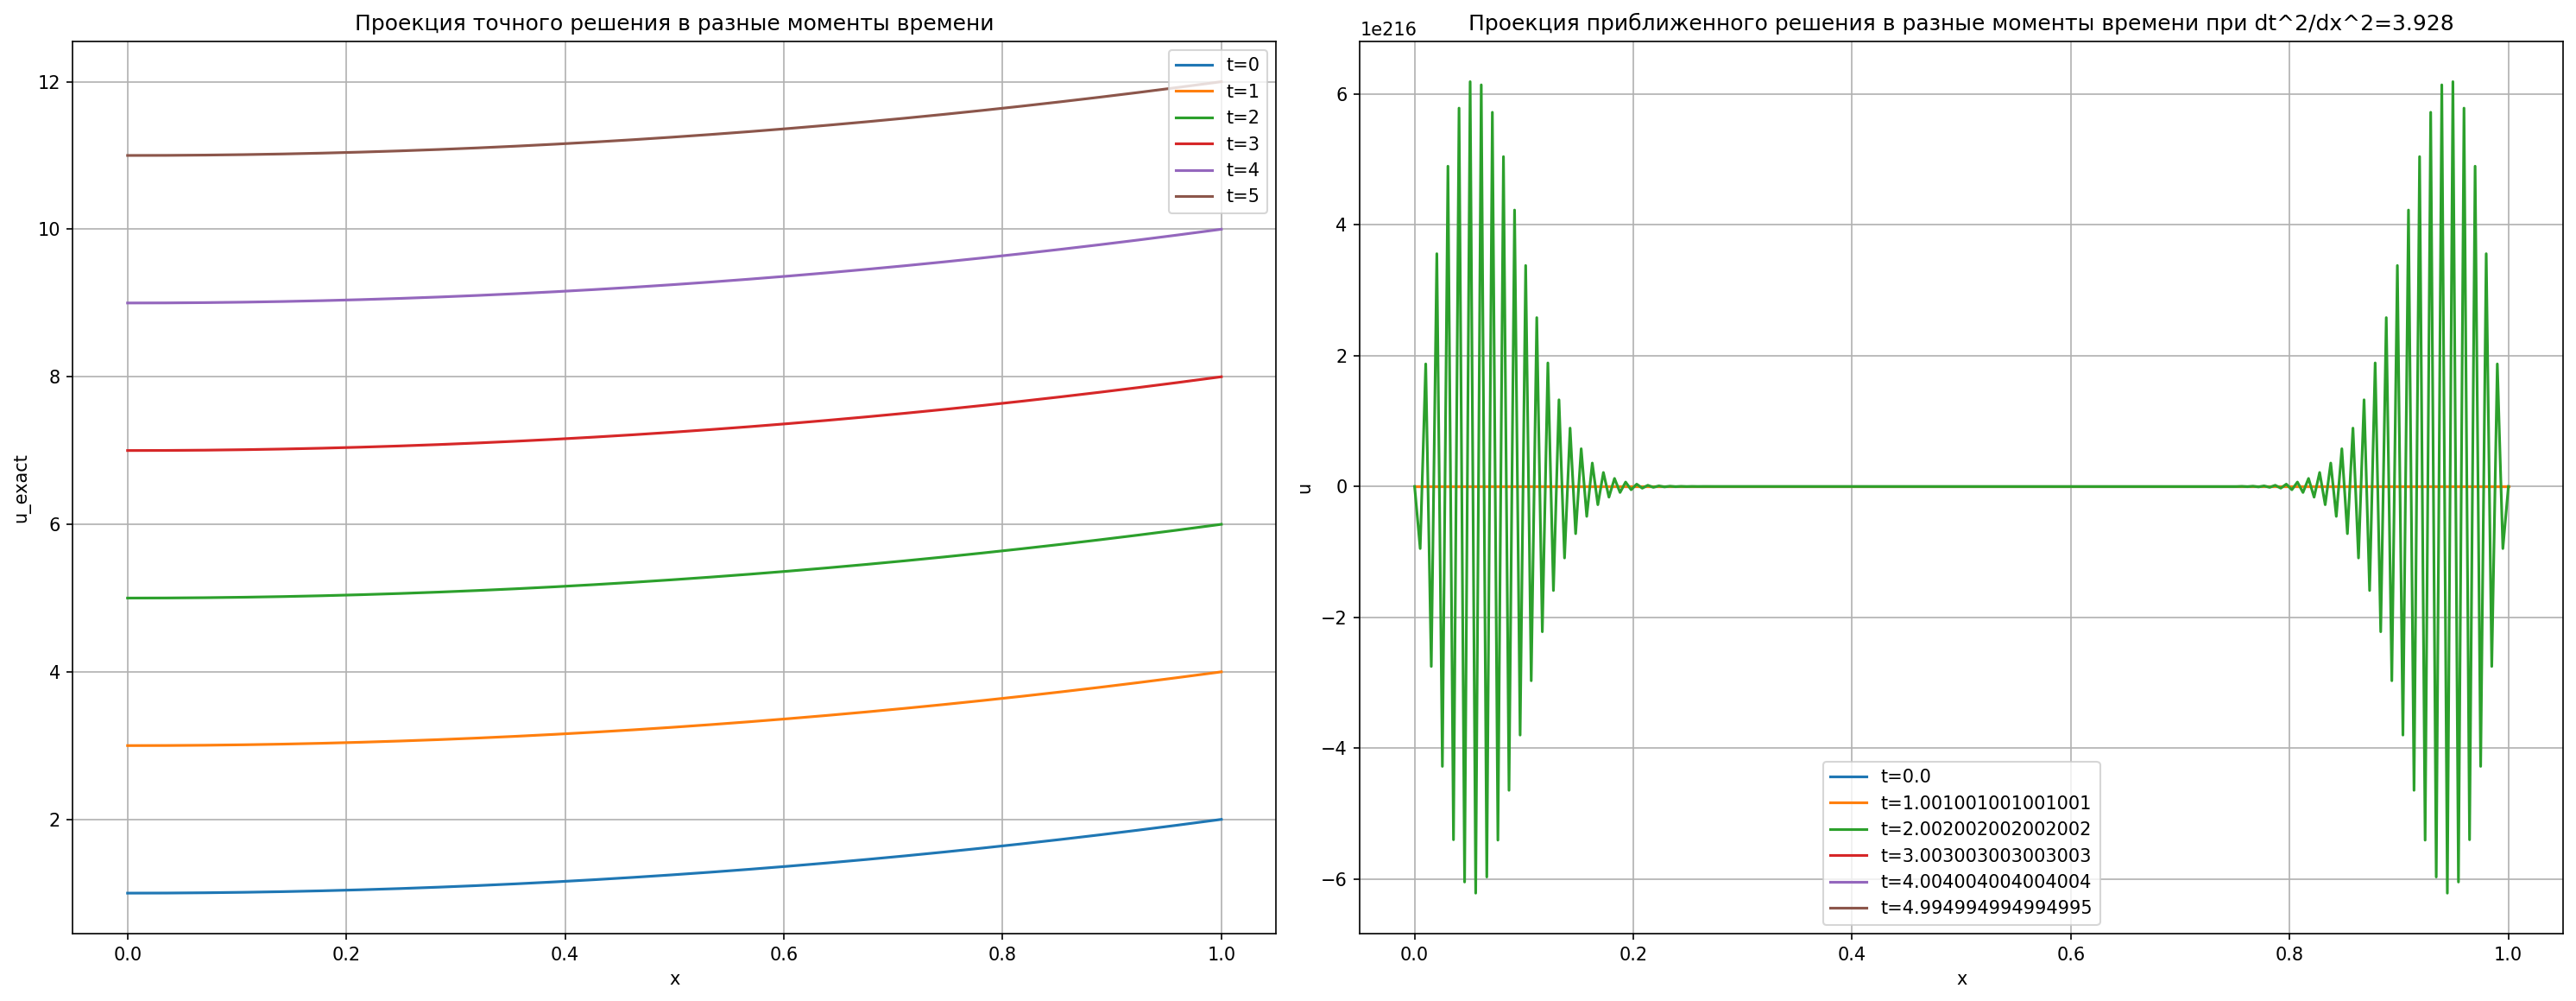
\includegraphics[width=0.45\textwidth]{figures/unstable_dt0_dx1.png}
\caption{$\tau = \tau_0$, $h = h_0/2$ (courant = 1.01)}
\label{fig:unstable1}
\end{figure}

\begin{figure}[H]
\centering
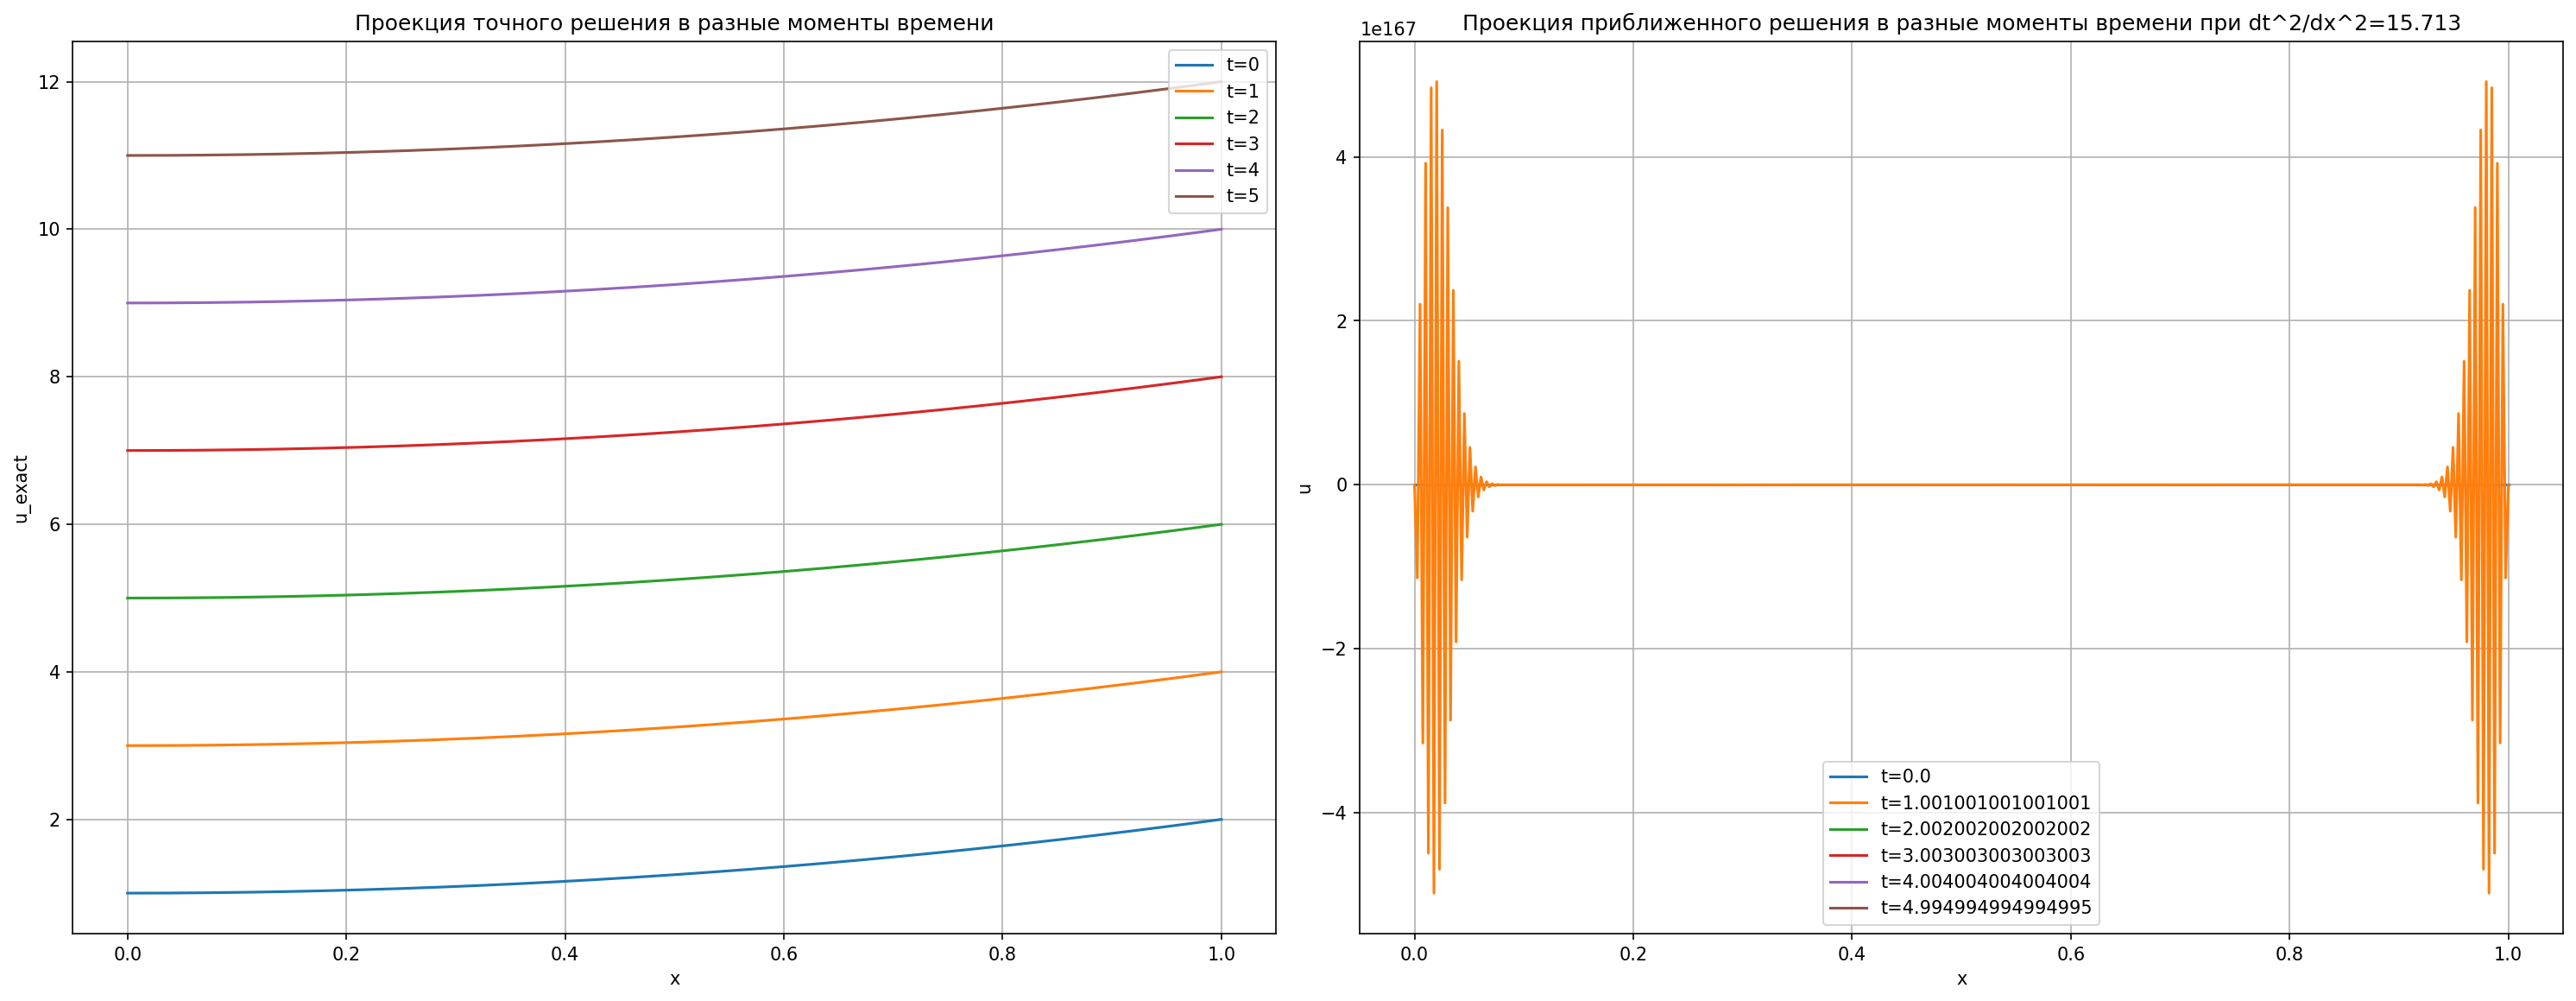
\includegraphics[width=0.45\textwidth]{figures/unstable_dt0_dx2.png}
\caption{$\tau = \tau_0$, $h = h_0/4$ (courant = 4.04)}
\label{fig:unstable2}
\end{figure}

\begin{figure}[H]
\centering
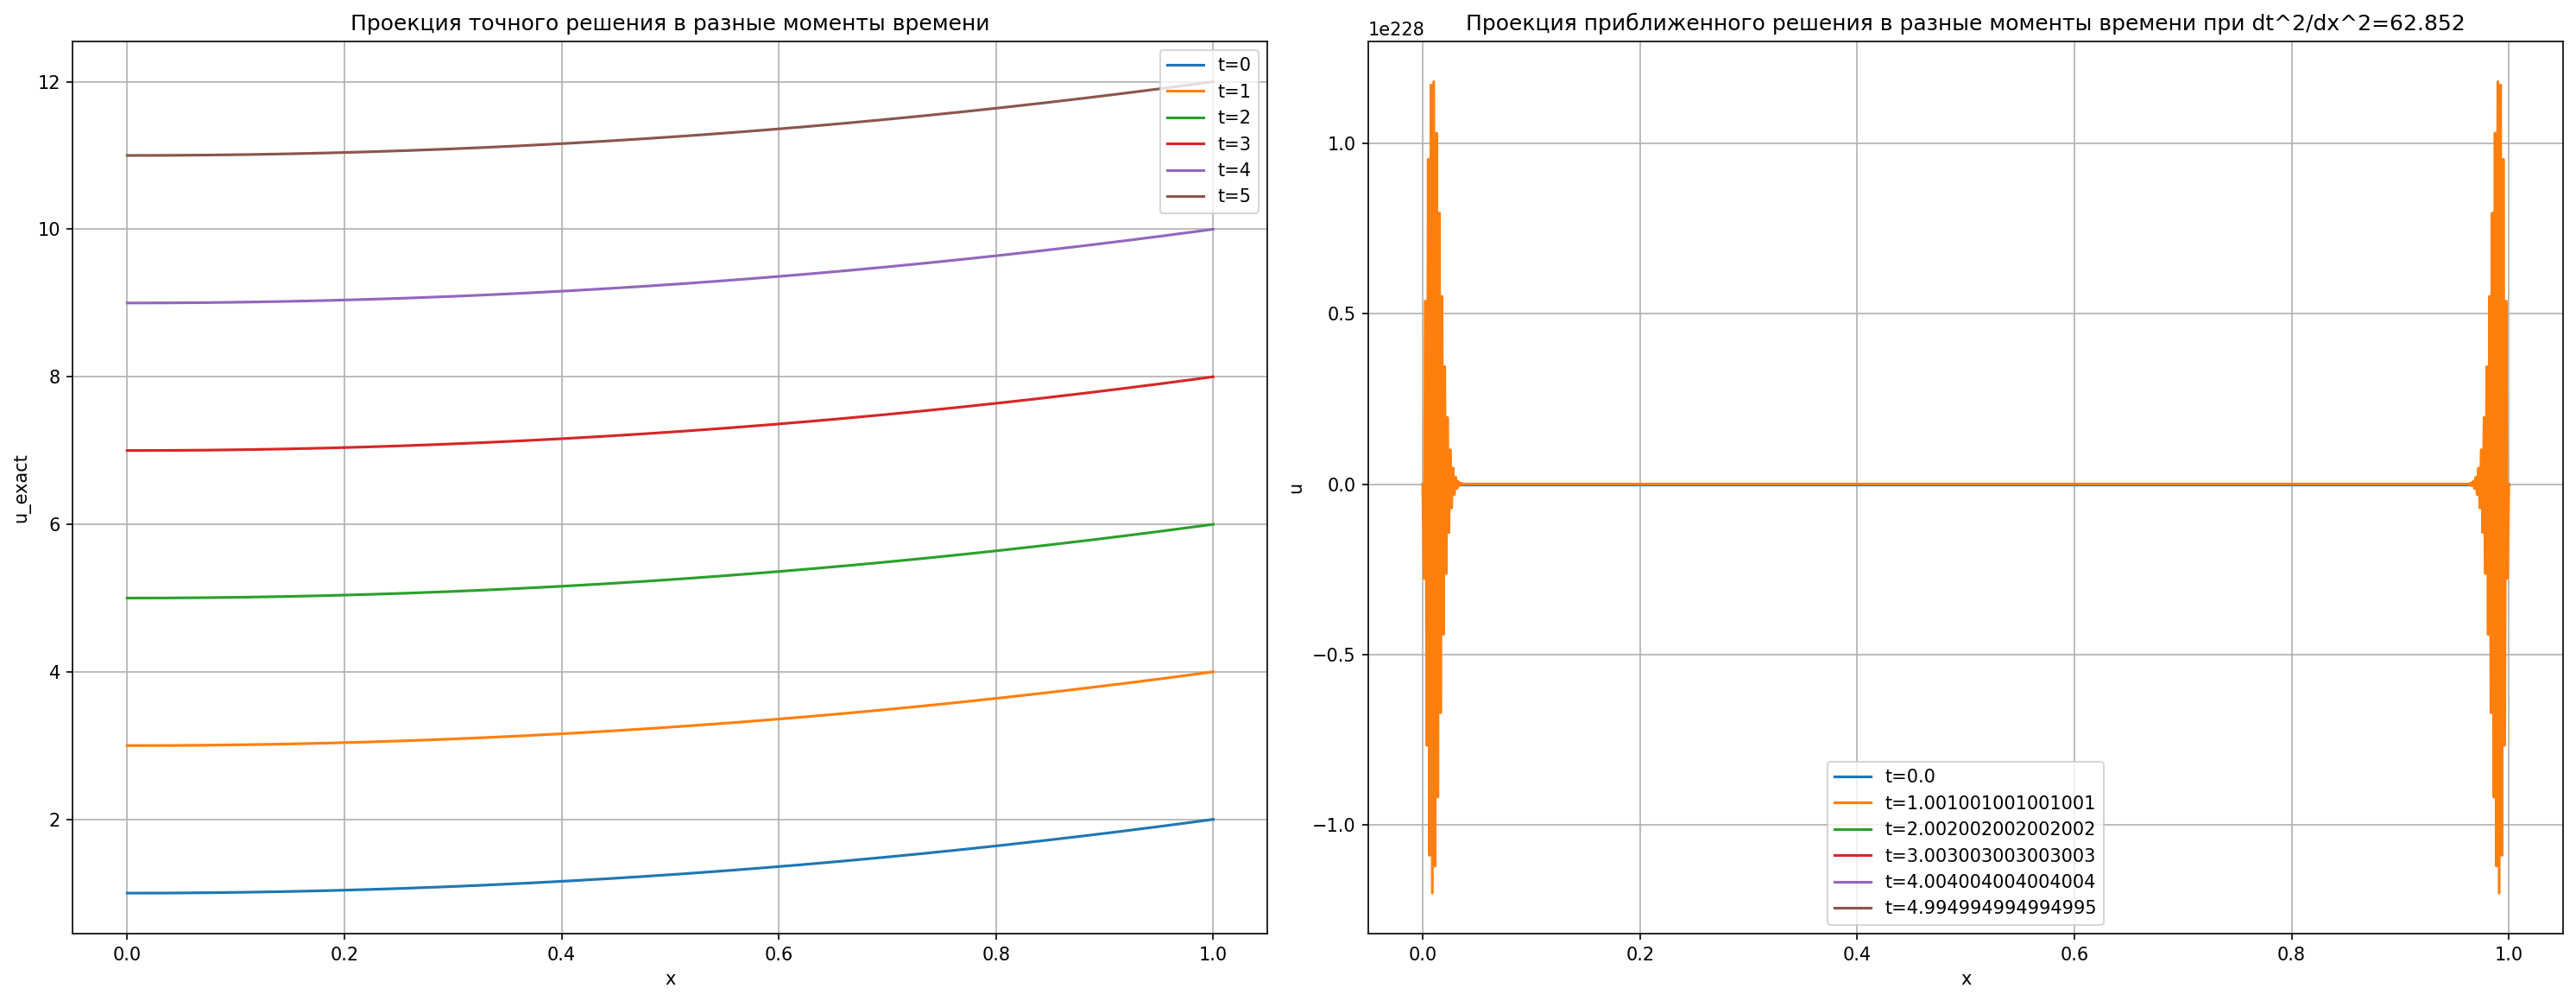
\includegraphics[width=0.45\textwidth]{figures/unstable_dt0_dx3.png}
\caption{$\tau = \tau_0$, $h = h_0/8$ (courant = 16.16)}
\label{fig:unstable3}
\end{figure}

\begin{figure}[H]
\centering
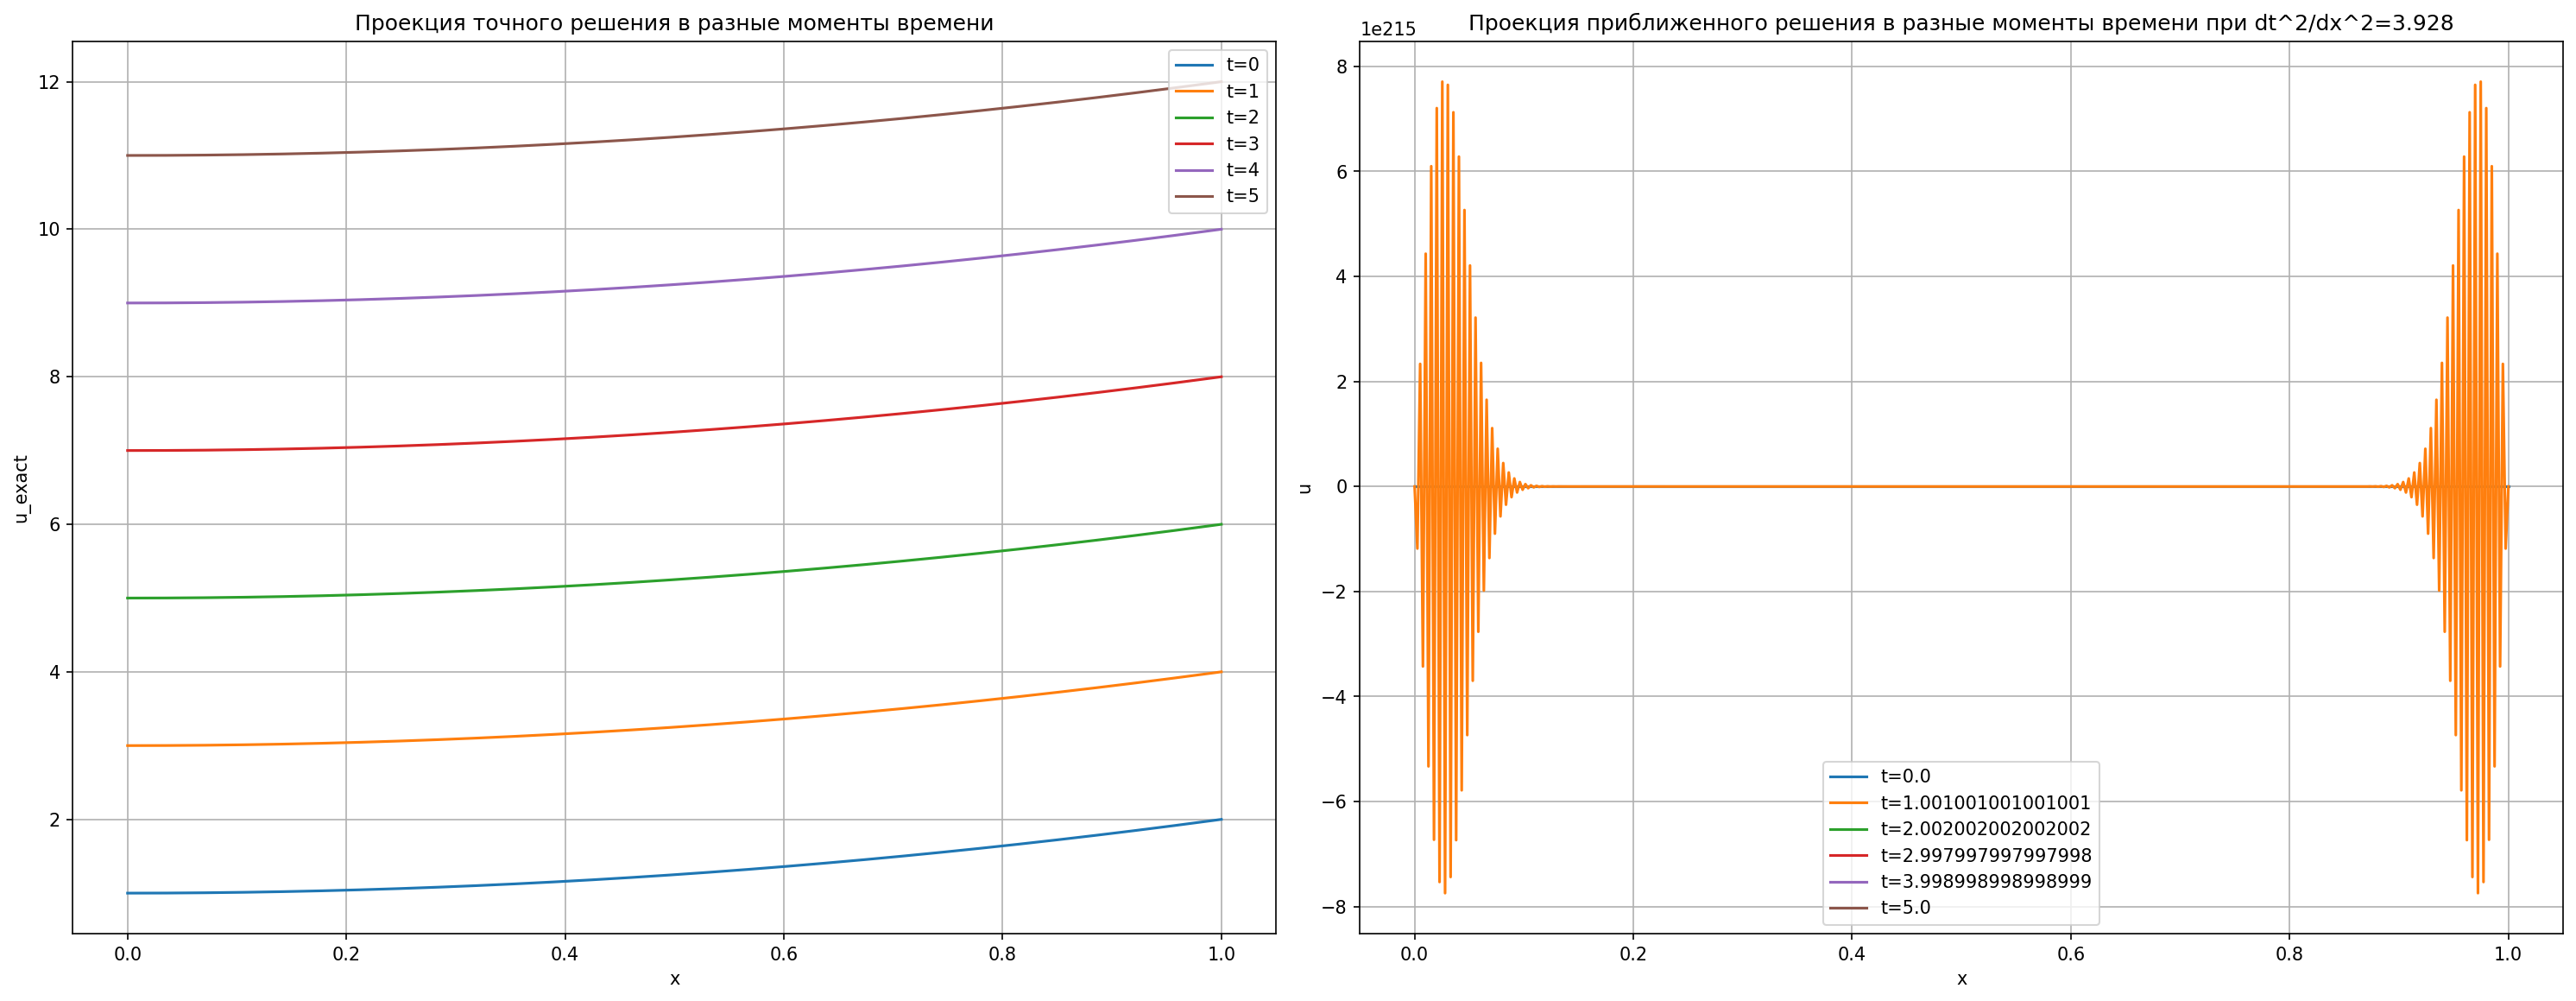
\includegraphics[width=0.45\textwidth]{figures/unstable_dt1_dx2.png}
\caption{$\tau = \tau_0/2$, $h = h_0/2$ (courant = 0.252) — устойчиво}
\label{fig:unstable4}
\end{figure}

\begin{figure}[H]
\centering
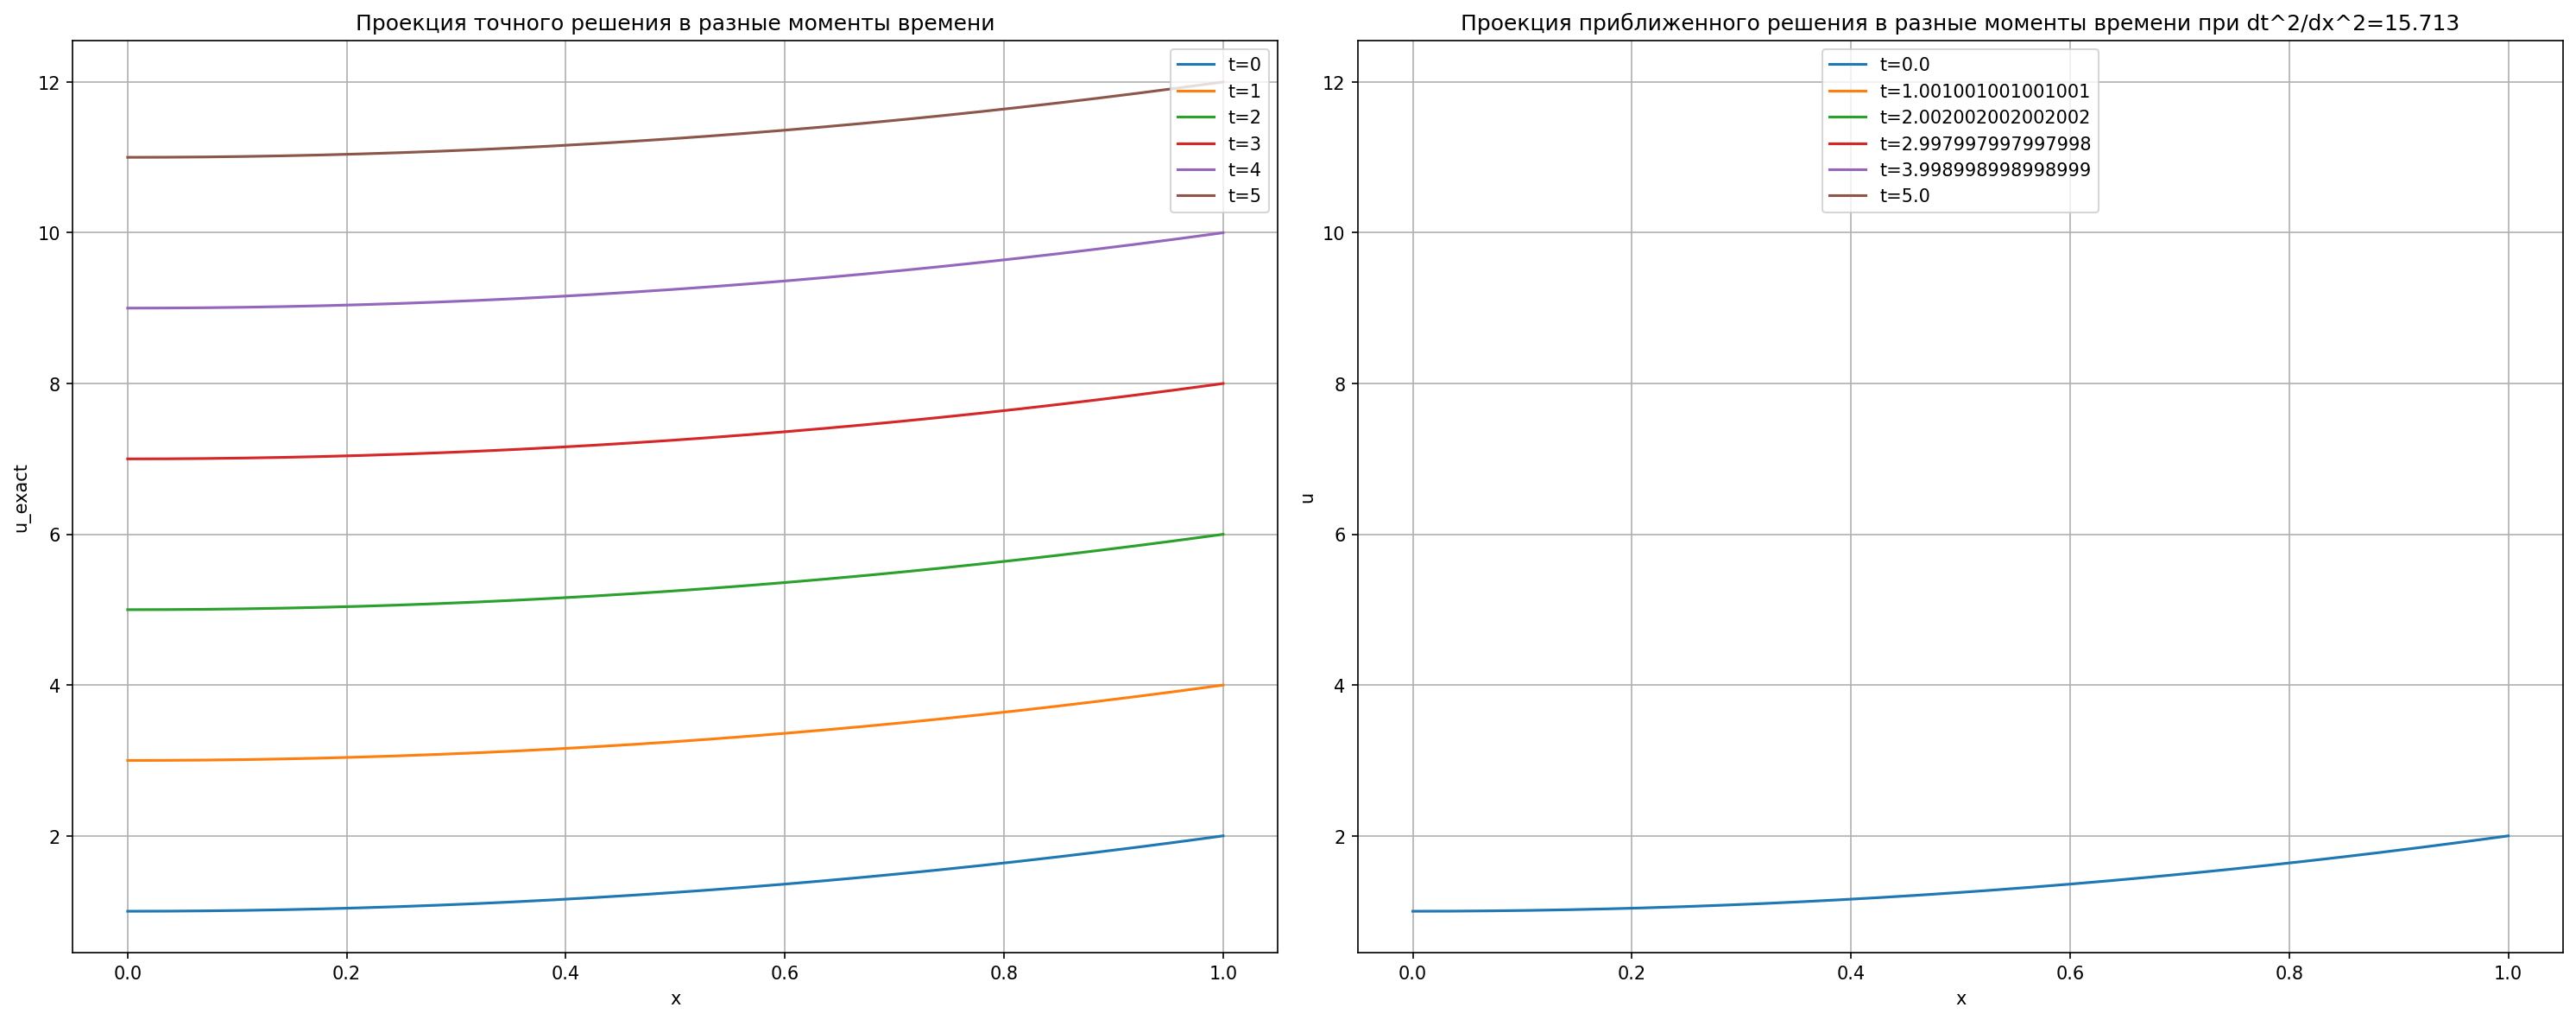
\includegraphics[width=0.45\textwidth]{figures/unstable_dt1_dx3.png}
\caption{$\tau = \tau_0/2$, $h = h_0/4$ (courant = 1.01)}
\label{fig:unstable5}
\end{figure}

\begin{figure}[H]
\centering
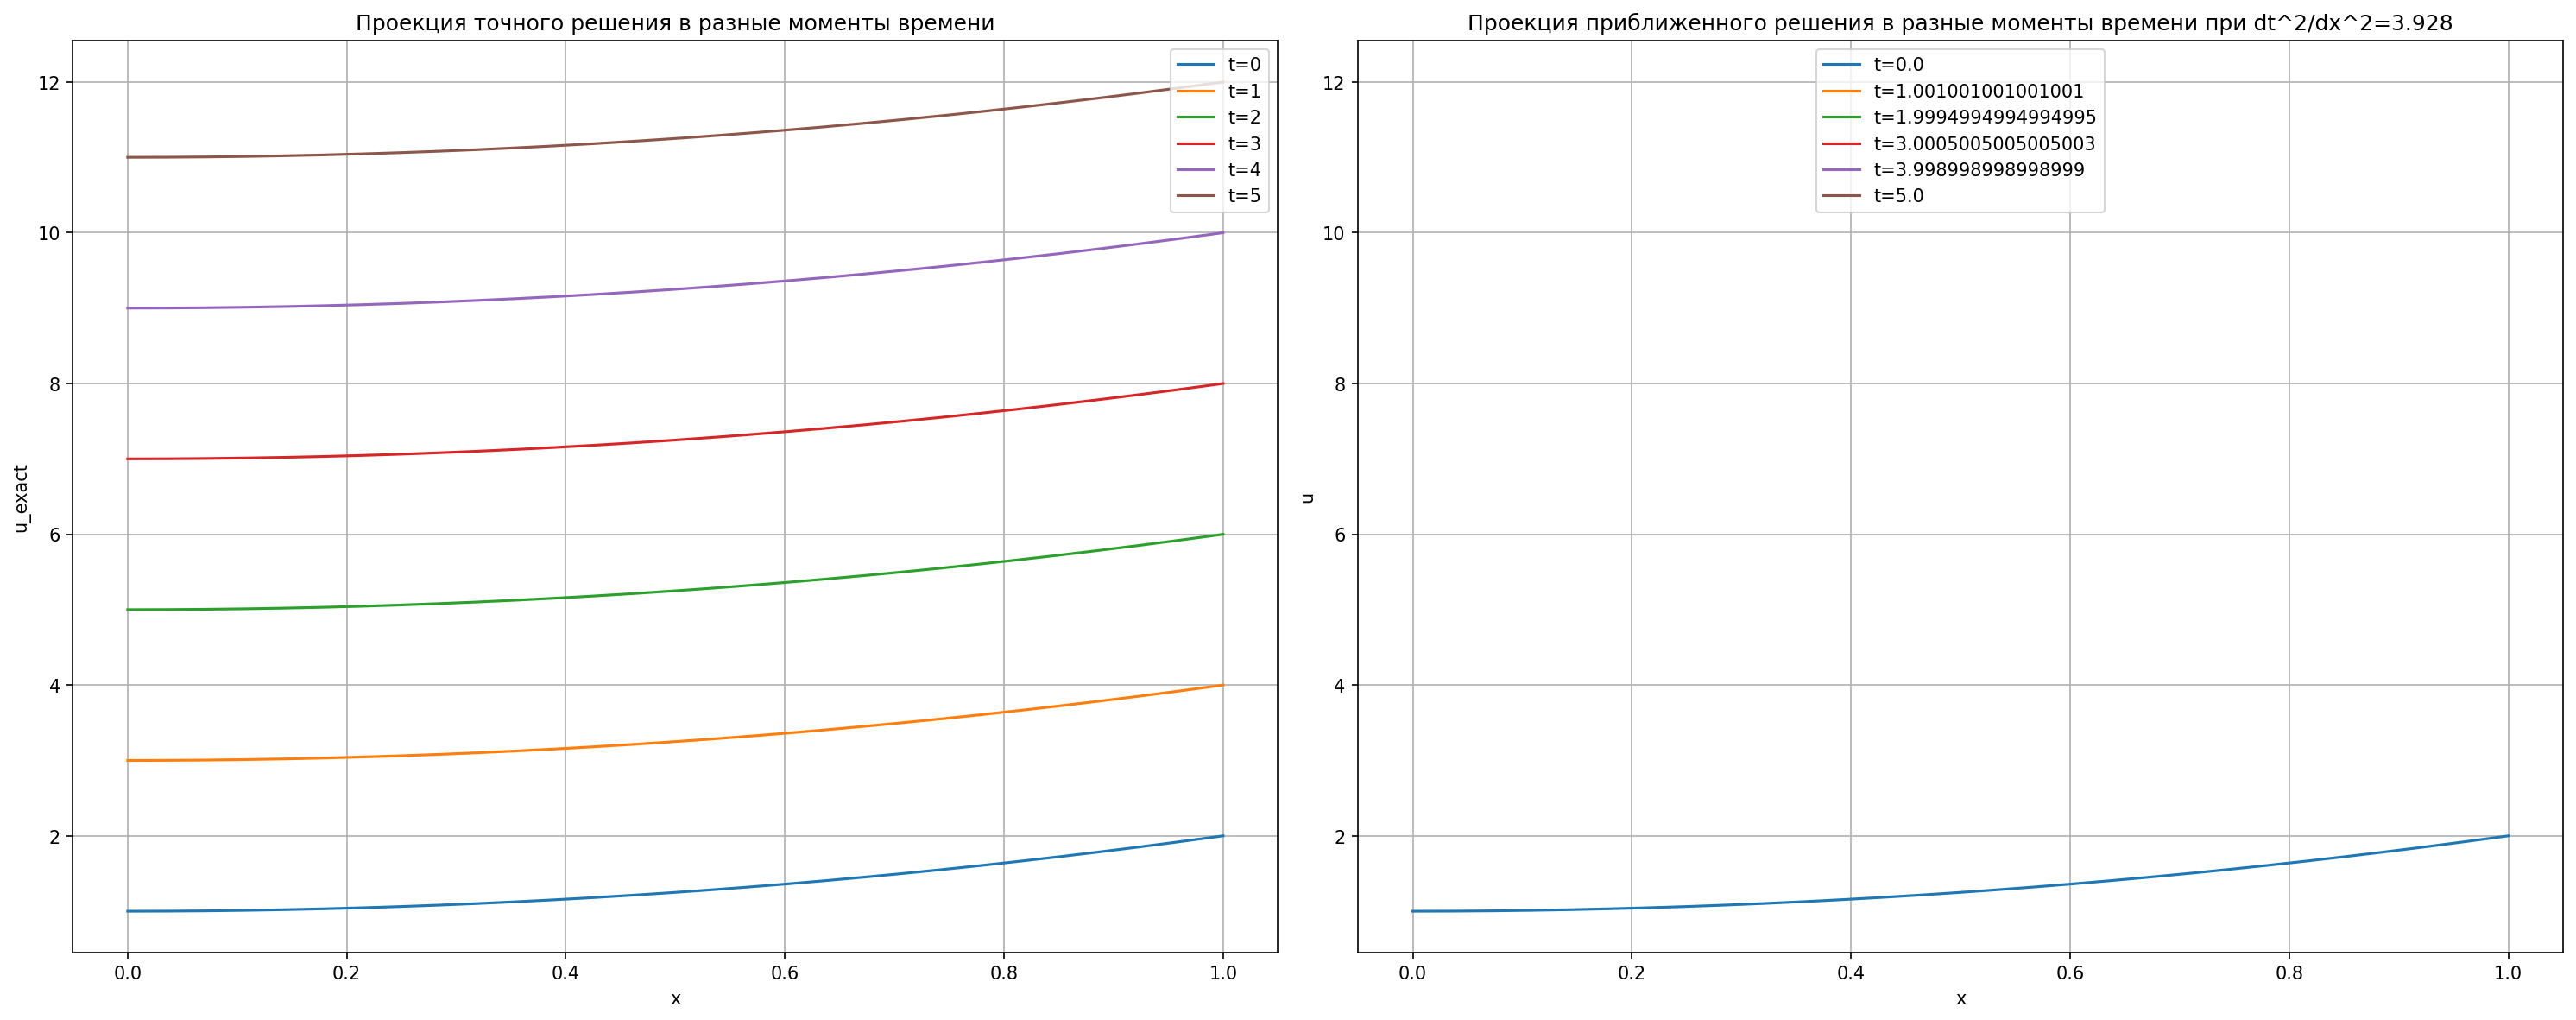
\includegraphics[width=0.45\textwidth]{figures/unstable_dt2_dx3.png}
\caption{$\tau = \tau_0/2$, $h = h_0/8$ (courant = 4.04)}
\label{fig:unstable6}
\end{figure}

\section{Выводы}

На основе проведенных численных экспериментов можно сделать следующие выводы:

\begin{enumerate}
    \item Разностная схема "Крест" реализована корректно — численное решение совпадает с точным с машинной точностью для тестового примера.
    \item Схема является условно устойчивой. При выполнении условия $\tau^2/h^2 < 1$ решение устойчиво, при нарушении — происходит разрушение решения (появление высокочастотных осцилляций и неограниченный рост амплитуды).
    \item Полученные результаты соответствуют теоретическим свойствам схемы.
\end{enumerate}

\end{document}